\documentclass[12pt]{article}
\usepackage{amsmath, amsfonts, fullpage, graphicx}
\usepackage[colorlinks]{hyperref}
\usepackage{algorithm}
\usepackage{algpseudocode}

\begin{document}

\section{Introduction}
\label{Introduction}

Community detection is an important graph problem with various applications.
This problem requires finding \textit{communities} of nodes on a graph. Ideally,
all nodes in a community should be similar according to some metric. Community
detection is an interesting problem because there is no obvious metric for
what makes a particular community assignment ``good'' or ``bad''; it must be
defined for the specific type of graph.

In this paper we present a fast, unsupervised community detection algorithm for
knowledge graphs. An overview of knowledge graphs is provided in section
\ref{Knowledge Graph Overview}. These graphs represent information as a set of
\textit{entity-relation triples} in the form $\langle e_1,\,r,\,e_2 \rangle$
where $e_1,e_2$ represent entities and $r$ represents the relation between them.
The collection of triples is the \textit{knowledge base}. Knowledge graphs can
have very specialized information (e.g. representing biological processes) or
very general information. Knowledge graphs are typically represented as one node
per entity and the relations as edge types between entities.

Previous work in community detection has focused on very general types of
graphs. This research is covered in Section \ref{Related Work}. Knowledge graphs
are simply the graph representation of a set of entity-relation triples and
therefore have a specific inherent structure. We take advantage of this
structure to create an algorithm that is faster than the general community
detection algorithms. Specifically, we convert the knowledge graph to a
bipartite representation. Details of the conversion are specified in Section
\ref{Bipartite Representation}. A bipartite representation allows the algorithm
to be fast while also benefiting from the very rigid structural rules of
bipartite graphs.

Community detection is a very important problem for knowledge graphs. A good
community detection algorithm provides insight into the structural properties of
the knowledge graphs. It can help clarify which types of nodes there are and how
many of each type. If we frame it as a machine learning problem, then growing
the knowledge base by adding new triples can be considered as an inference
problem. Once we understand the breakdown of the existing graph, the entities
and relation in the new triple can be easily categorized, providing information
about the nodes beyond the simple textual information of the triple
itself.Community detection on a knowledge graph also has applications to various
other graph problems, such as question answering and social network analysis. By
understanding the knowledge graph we can more easily answer queries about the
knowledge graph. Similarly, most general network graphs can be converted into
knowledge graphs. Thus a community detection algorithm can find patterns in
social networks as well.

Many knowledge graphs such as Freebase\cite{Freebase} have millions of triples.
Traditional community detection algorithms are $O(n^2 \log n)$ or $O(n^2)$,
which is not computationally feasible for large datasets. The algorithm
presented here is almost linear, which allows it to scale to large datasets. The
speed of the algorithm allows it to generalize to any knowledge graph datset.The
algorithm is also completely unsupervised, which is not the case for most
knowledge graph
algorithms\cite{Nickel2011}\cite{Bordes2013}\cite{Gao2015}\cite{Chang2014}.
Since community detection is such a hard problem with no obvious answer, an
unsupervised algorithm learns to detect any pattern in the graph. It can even
detect patterns that the humans might not have been able to see. On the other
hand, a supervised algorithm can only learn from the specific type of
supervision given as feedback.

The structure of the paper is as follows. We first provide a quick overview on
knowledge graphs. Then we review related work in the areas of community
detection and knowledge graph analysis. Aftewards we present the bipartite
representation of knowledge graphs and the mathematical details of the
algorithm. Finally we present our results on the NELL\cite{Carlson2010}
knowledge graph dataset.

\section{Related Work}
\label{Related Work}

Community detection is a problem that has been studied quite extensively.
Kernighan and Lin\cite{Kernighan1970} created one of the first algorithms.
The algorithm we present here is loosely based on it. Their algorithm works by
partitioning the graph into two sections, choosing how to move nodes to maximize
some benefit function, and then picking the state which has maximum benefit.

Newman\cite{Newman2004} presents a comprehensive survey on the field of
community detection. He discusses the Kernighan-Lin algorithm as well as the
Girvan-Newman algorithm\cite{Girvan2002}.

Many algorithms have focused on the stochastic blockmodel\cite{Holland1983}.
Karrer and Newman\cite{Karrer2011} presented a modified version of this algorithm
which iteratively moves nodes from one community to another in order to maximize
some objective function. This is the inspiration for the algorithm presented here.
Larremore et al.\cite{Larremore2014} extend Karrer and Newman's method to a bipartite
graph to obtain speedup. Their work serves as the basis for our algorithm, which
converts the knowledge graph to a bipartite representation.

Much research has been done with knowledge graphs as well, but none in the area
of community detection on the original graph. Bordes et al.\cite{Bordes2013}
provide a way to embed the knowledge graph using neural networks, and Gao et
al.\cite{Gao2015} improve that model by enforcing Semantically Smooth Embedding.
Nickel et al.\cite{Nickel2011} propose a model for embedding using tensor decomposition
instead. Chang et al.\cite{Chang2014} improve the runtime of the Nickel model to
make it more computationally feasible.

\section{Knowledge Graph Overview}
\label{Knowledge Graph Overview}

A knowledge graph generally refers to a set of \textit{entity-relation triples}.
These triples take the form $\langle e_1, r, e_2 \rangle$. where $e_1$ and $e_2$
are entities and $r$ describes the relation between these two entities. Entities
and relations can be repeated across triples. The total set of triples denotes
all the knowledge in our ``Knowledge Base''.

\begin{figure}[t!]
    \centering
    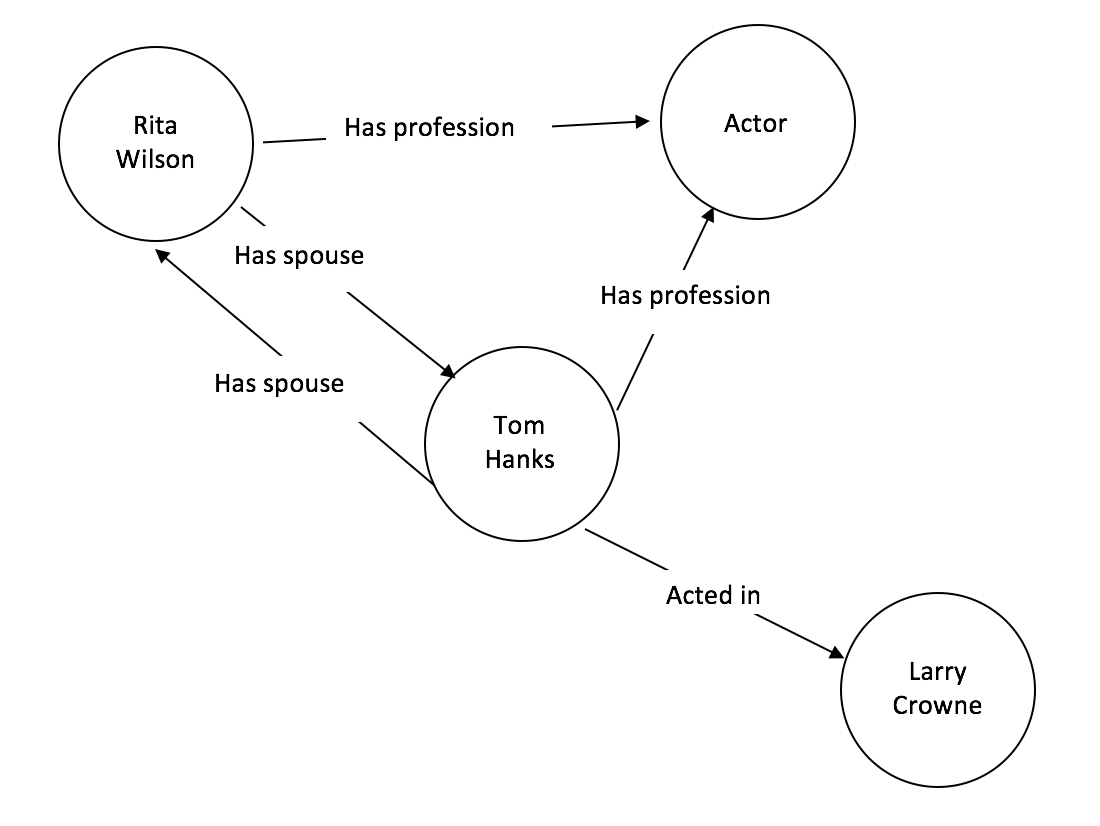
\includegraphics[width=0.7\textwidth,keepaspectratio]{figures/Example_KG.png}
    \caption{A small example knowledge graph}
    \label{fig: Example_KG}
\end{figure}

We can represent these triples as a directed graph, with each entity as a vertex
and the relations as edge types between them. Figure \ref{fig: Example_KG} shows
an example of a very small knowledge graph. Note that there is only one node per
entity. This allows the graph to store multiple pieces of information regarding
the same entity together, to allow for easy processing by the program while also
making it simple for humans to understand.

Once a knowledge graph is built, we can pose queries about the graph. For
example, we can provide two entities $e_1$, $e_2$ and ask which relation $r$
links the two on the graph. We can also provide an entity $e$ and the relation
$r$, and ask for which other entity $e'$ do the triples $\langle e,r,e' \rangle$
or $\langle e',r,e \rangle$ exist on the graph. Put another way, the queries are
either \textit{link prediction} queries or \textit{entity prediction} queries.

\section{Bipartite Representation}
\label{Bipartite Representation}

We propose converting the knowledge graph into a directed bipartite
representation to help perform the task of community detection. In this form,
all entities belong to one \textit{class} while all relations belong to the
other class. Figure~\ref{fig: Bipartite_KG} shows the graph in Figure~\ref{fig: Example_KG}
converted to a bipartite representation.

\begin{figure}
    \centering
    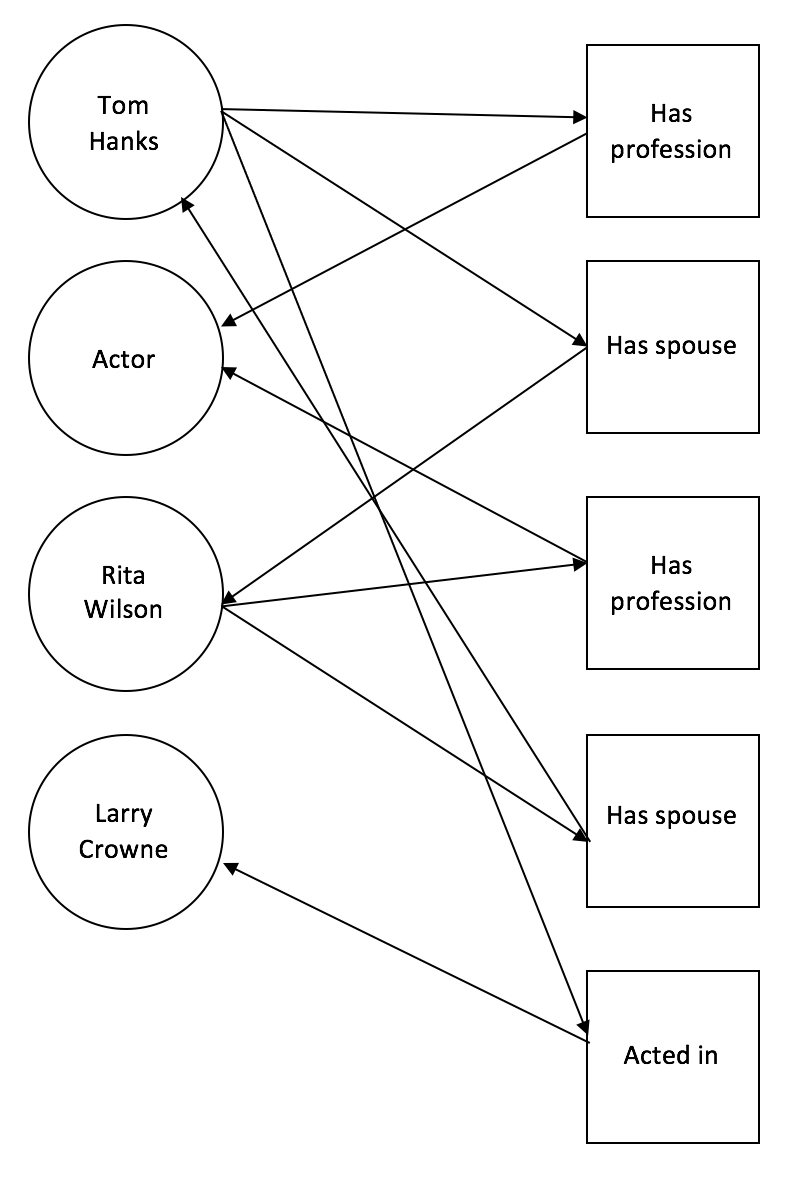
\includegraphics[width=0.7\textwidth,keepaspectratio]{figures/Bipartite_KG.png}
    \caption{A bipartite representation of the graph in Figure~\ref{fig: Example_KG} }
    \label{fig: Bipartite_KG}
\end{figure}

The conversion is done as follows. Consider some triple $\langle e_1,\,r,\,e_2
\rangle$. There is still exactly one node for each entity, regardless of how
many triples that entity appears in. Thus we have one node $e_1$ and another
$e_2$. We also make a node for $r$, which we call the \textit{relation node}. We
then add a directed link from $e_1$ to $r$, and a directed link from $r$ to
$e_2$. It is important to note that we make a separate node for each occurence
of a relation. Thus if there is another triple $\langle e_3,\,r,\,e_4 \rangle$
then we would make a separate node for $r$, even though the relation type itself
is the same. As a result, every relation node has exactly one inbound and one
outbound edge. Each entity node, on the other hand, has the same outbound and
inbound edges as in the original graph. The number of relation nodes is exactly
equal to the number of triples, since we add one relation node for every triple.

There are several advantages to using a bipartite representation. The algorithm
presented here is unsupervised, so there is no input besides the graph itself.
The communities can only be found using the distribution of nodes and edges.
Therefore, the stronger an inherent structure can be provided as input, the
better the algorithm will do. Bipartite graphs enforce a very rigid structure on
the graphs, more so than almost any other graph representation. This means that
we provide our algorithm with a rigid structure.

This structure in turn creates a natural way to find communities of nodes. By
partitioning into entity nodes and relation nodes, we only have to focus on
nodes of one class when finding communities, i.e. communities with entity nodes
will only have entity nodes, and similarly for relation nodes. Additionally, we
define these communities \textbf{based on links to nodes of the opposite class}.
That is to say, entities that have outbound links to the same types of relations
and inbound edges from the same types of relations should be in the same
community. Similarly, relation nodes that have inbound links from entity nodes
of the same community and outbound links to entity nodes of the same community
are probably the same type of relation.

Figure~\ref{fig: Colored_Bipartite_KG} shows a possible community assignment of
the graph in Figure~\ref{fig: Bipartite_KG}, where each color represents a
different community. \textit{Tom Hanks} and \textit{Rita Wilson} both have an
outbound edge to the gray community, which represents the \textit{has
profession} relation. Both also have inbound edges from the \textit{has spouse}
relation. Since both have outbound edges to the same type of relation community
and inbound edges from the same type of relation community, the algorithm should
place these two entities in the same community. On the other hand,
\textit{Actor} only has inbound links from the \textit{has profession}
community, so it should be in a separate community from \textit{Tom Hanks} and
\textit{Rita Wilson}.

\begin{figure}
    \centering
    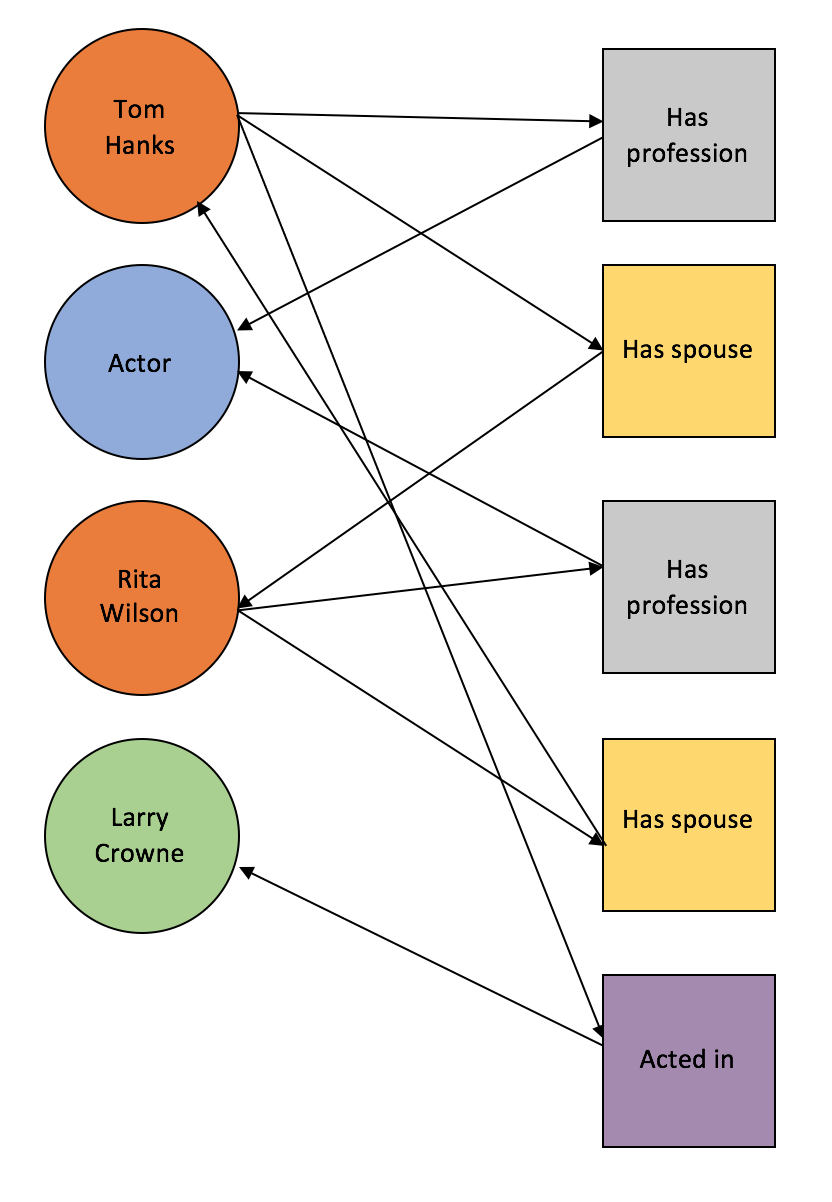
\includegraphics[width=0.7\textwidth,keepaspectratio]{figures/Colored_Bipartite_KG.png}
    \caption{A possible community assignment of the graph in Figure~\ref{fig: Bipartite_KG} }
    \label{fig: Colored_Bipartite_KG}
\end{figure}

Communities defined this way can be detected for one class independently of the
other class, allowing for parallelization and therefore decreasing the running
time of the program. As discussed in Section \ref{Related Work}, previous
community detection algorithms are $O(n^2\lg n)$ or $O(n^2)$, often because they
have to perform a linear check over all nodes for each node they visit. However,
the bipartite structure means that we can operate on the entity nodes and
relation nodes independently, significantly lowering our runtime. The full
analysis is discussed in Section \ref{Time Analysis}.

A third advantage of the bipartite representation is that in converting the
relations to nodes, every edge in the resulting graph is untyped. Each edge can
be processed in the same way. Additionally, the resulting adjacency tensor for
the graph has only two dimensions, instead of the three-dimensional tensor used
by Nickel et al.\cite{Nickel2011} and Chang et al.\cite{Chang2011}. As edges
are untyped, there does not need to be a separate matrix for each type $k$.

\section{Model}
\label{Model}

\subsection{Algorithm Overview}
\label{Algorithm Overview}

Section \ref{Bipartite Representation} provided the intuition for our algorithm.
In this section we formalize the details. Algorithm \ref{alg: main_alg} shows
the pseudocode for the algorithm. Let $K_e$ be the set of entity communities and
$K_r$ the set of relation communities. We specify $|K_e|$ and $|K_r|$
beforehand. We read in the knowledge graph data and create the bipartite
representation with $E$ the set of entity nodes and $R$ the set of relation
nodes, and $N_e = |E|,\,N_r = |R|$. Note that $N_r$ is the number of triples
in the set, since we have one relation node for every triple.
% For convenience,
% let $e$ be the number of entity nodes and $a$ the number of relation nodes.
The
input data also provides us with $O$ and $A$, the outbound and inbound adjacency
matrices, respectively. Each of these is a binary $N_e\times N_r$ matrix, where
$O_{ij} = 1$ if and only if edge there is a directed edge $e_{ij}$ from entity
node $i$ to relation node $j$, and $I_{ij}$ is the same but for an edge from
relation node $j$ to entity node $i$.

\begin{algorithm}[t!]
\caption{Community Detection Algorithm}\label{alg: main_alg}
\begin{algorithmic}[1]

\Function{Detect-Communities}{$E, R, |K_e|, |K_r|, max\_iter, O, I, \epsilon$}
    \State $state\_pen, l, L, K_e, K_r\gets \Call{Initialize}{E, R, |K_e|, |K_r|, O, I}$
    \State $iter\gets 0$
    \While{$iter < max\_iter$ or $state\_pen < \epsilon$}
        \State $move\_e\gets \Call{Entity\_Penalties}{E, K_e, l, L}$
        \State $move\_r\gets \Call{Relation\_Penalties}{R, K_r, l, L}$
        \State $K_e,K_r\gets \Call{Move\_And\_Update}{move\_e, move\_r, K_e, K_r, l, L}$
        \State $state\_pen\gets \Call{State\_Penalty}{K_e, K_r, l, L}$
    \EndWhile
    \State \textbf{return} $K_e, K_r$
\EndFunction

\end{algorithmic}
\end{algorithm}

The algorithm is iterative. Each node is assigned a penalty score based on how
its outbound/inbound edges differ from the other nodes in its community. In each
iteration, we pick the entity node and relation node with the highest penalty
and assign them to the community in which they have lowest penalty. We also
define a total state penalty as the sum of all node penalties. The algorithm
continues iterating until the total state penalty is within some tolerance or
until some fixed \textit{max\_iterations}.

For convenience in our analysis we will focus only on the outbound matrix $O$,
and on entity nodes/communities. The analysis for the inbound matrix is the
exact same. To analyze outbound/inbound edges for the relation nodes we take the
transpose of the opposite matrix. The outbound adjacency matrix for relation
nodes is $I^T$, and the inbound matrix is $O^T$.

First consider an entity node $i$ and a relation community $r$. Let
$l_{ir,outbound}$ be the total number of outbound edges from $i$ to any relation
node in $r$. We can store these quantities in the $N_e\times |K_r|$ matrix
$l_{outbound}$.

$$l_{ir, outbound} = \sum_{j \in r} O_{ij}$$

We can extend this analysis to inter-community links. Consider an entity
community $c$. Let $L_{cr,outbound}$ be the number of outbound edges between $c$
and relation community $r$. This is just the sum of outbound edges from any node
in $c$ to any node in $r$. We can store these quantities in the $|K_e|\times
|K_r|$ matrix $L_{outbound}$.

$$L_{cr, outbound} = \sum_{i \in c} l_{ir, outbound} = \sum_{i \in c} \sum_{j \in r} O_{ij} $$

The intuition behind the penalty is that nodes in the same community should have
about the same number of outbound edges to each relation community and the same
number of inbound edges from each relation community. To frame it in the original
knowledge graph, nodes in the same community should be involved in similar relations.
If we assign two nodes to one community, and they are involved in very different
types of relations, then they should not be in the same community.

Let $d_{outbound}(c,r), d_{inbound}(c,r)$ be the average outbound/inbound links
from community $c$ to community $r$.

$$d_{outbound}(c,r) = \frac{L_{cr, outbound}}{|c|}$$

Now define the \textbf{node penalty} $p(i)$ of node $i$ as the squared difference
of the edges out from / into $i$ and the average links in $i$'s community $c$.

$$p(i) = \sum_{r \in K_r} (d_{outbound}(c,r) - l_{ir,outbound})^2 +
(d_{inbound}(c,r) - l_{ir, inbound})^2 $$

A given assignment of nodes to communities is a \textit{state}. The state penalty
$P(s)$ is simply the sum of each node penalty.

$$P(s) = \sum_{i \in E} p(i) + \sum_{j \in R} p(j)$$

How well the entity communities are formed depends on how accurate the relation
communities are, and vice versa. The algorithm is iterative so that entity and
relation communities can be slowly improved simultaneously. A better assignment
of entity communities will make the relation communities better, which will in
turn make the entity communities better.

Sometimes, certain states act as \textit{local minima}, in which moving the
entity and relation nodes with highest penalty would actually increase the state
penalty. If the total state penalty is below some tolerance then this is
actually a proper assignment of communities, but often the total state penalty
is still high. In this case we randomly choose which new community to assign
these nodes to. Due to the fact that improving each class of communities depends
on improving the other class of communities, these local minima arise when the
assignments are such that we reach an equilibrium point. Often they are a
consequence of the random initializations. Therefore, as with many randomized
algorithms, this algorithm is run many times with different initializations each
time.

\subsection{Similarity to other AI Algorithms}
\label{Similarity to other AI Algorithms}

The algorithm presented here is very similar to other algorithms in the field of
Artificial Intelligence. Essentially, we are treating the problem of community
detection as a search problem, where we try to find the optimal assignment
of nodes to communities given some constraints. In this case, the constraint is
to minimize the state penalty.

Our approach is a greedy one, where in each iteration the algorithm tries to
find the re-assignment of one entity node and one relation node such that
penalty is minimized. If the algorithm hits a local minimum, it randomly chooses
which communities to re-assign the nodes to. This approach is very similar to
that of  WALKSAT, an algorithm for finding boolean satisfiability. WALKSAT
greedily finds a variable assignment that satisfies the most unsatisfied
clauses, but with some probability does a random assignment every iteration to
avoid local minima.

\subsection{Runtime Analysis}
\label{Runtime Analysis}

One goal of the algorithm is to be faster than the $O(n^2)$ runtime of the
other community detection algorithms\cite{ohai}\cite{other}. As discussed in
Section \ref{Bipartite Representation}, the bipartite structure of the graph
allows us to run the algorithm for entities and relations simultaneously.

We can save computation by calculating the matrices $l_{outbound}, l_{inbound},
L_{outbound}, L_{inbound}$ for entities and relations right after
initialization. Then in each iteration, we only have to update these matrices
for the entity node and relation node that are moved.

Calculating $l_{i, outbound}$ for a node requires summing over all relation
nodes, so the total time to calculate $l_{outbound}$ is $O(N_eN_r)$, which is
the number of entity nodes times the number of relation nodes. Once the $l$
matrix is calculated, the $L_{outbound}$ matrix is simply the sum over each
entity node (since every node is assigned to exactly one community). Thus
calculating $L_{outbound}$ takes $O(N_e)$ time (and $O(N_r)$ time when
calculating for the relation side). Our total precomputation is dominated by the
$O(N_eN_r)$ term.

In each iteration, calculating the penalty score of an entity node requires summing
over every relation community, which is $O(|K_r|)$ time. Finding the penalty of
a relation node takes $O(|K_e|)$ time. Finding the entity node with highest
penalty therefore takes $O(N_e|K_r|)$ time, and finding the relation node with
highest penalty is $O(N_r|K_e|)$.

Finding the optimal community to move to requires calculating the node's penalty
in each community. This is $O(|K_e||K_r|)$ for both the entity node and relation
node.

Finally, moving the node requires updating all nodes of the opposite class that
it is connected to. This takes $O(N_r)$ time for the entity node and $O(1)$ time
for the relation node, since each relation node has only 2 edges.

The total time per iteration is dominated by finding the nodes with highest
penalty. Therefore we spend $$O(N_e|K_r| + N_r|K_e|)$$ time per iteration.
The total number of nodes is $N_e + N_r$, and $|K_e| << N_e,\,|K_r| << N_r$.
The algorithm is not quite linear but almost linear per iteration, which means
that it is a fast algorithm relative to other community detection algorithms.
Lower runtime allows the algorithm to scale up to very large datasets.

\section{Results}
\label{Results}

In this section we present our results on the NELL dataset\cite{Carlson2010}.
The algorithm was implemented in Python using Numpy\cite{Jones2001} and Jupyter
Notebook\cite{Perez2007}. We first take in the NELL input in triple format and
convert it to the bipartite representation. We then run the algorithm on the
bipartite graph.

The Never Ending Language Project (NELL) is a project at Carnegie Mellon which
parses human knowledge from the Internet and generates entity-relation triples.
We use the NELL 165 version. It is possible that the triple is not actually
true, but that does not matter for the algorithm. We run two experiments on the
dataset.

The first is a very small proof-of-concept experiment with only one relation
type. The relation side acts as a control while the entity communities
demonstrate whether the algorithm can actually assign communities properly. We
use a set of eight triples, all of the form $\langle \text{event},
\,\text{eventdate}, \,\text{date}$. In each of these triples, $e_1$ is some
historical event and $e_2$ is its associated date. An optimal community
assignment is shown in Figure~\ref{fig: events} for two triples. If we specify
$|K_e| = 2$ and $|K_r|=1$ then the best way to assign communities for this set of
triples is to assign all events to one community and all dates to the other. We
expect the algorithm to do this as well, because events will have only outbound
edges to the single relation community and dates will have only inbound edges.

\begin{figure}[t!]
    \centering
    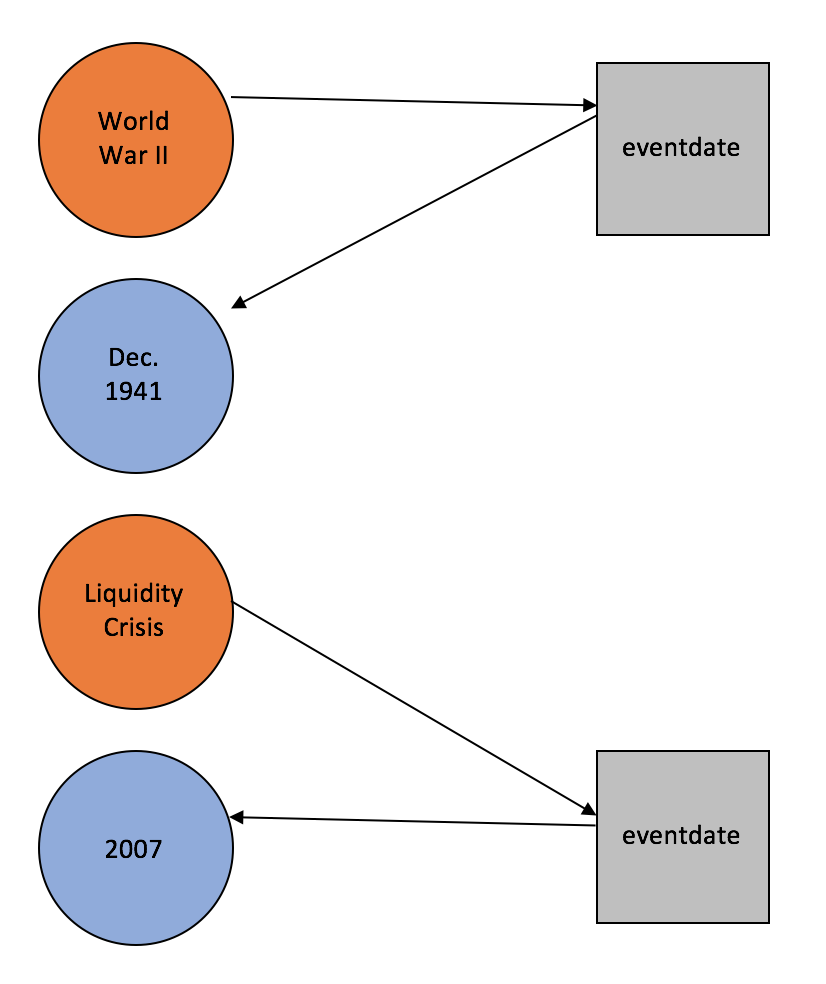
\includegraphics[width=0.7\textwidth,keepaspectratio]{figures/event_example.png}
    \caption{An optimal community assignment for two triples from the Events set}
    \label{fig: events}
\end{figure}

Table~\ref{tab: events} shows the result of running the algorithm on this small
dataset. The algorithm does perfectly split the 8 triples, with only dates in
Community 1 and only events in Community 2. That the algorithm is able to find
the optimal partition here indicates it could yield promising results on more
complicated datsets.

\begin{table}[b]
    \begin{tabular}{|c|c|}
        \hline
        Community 1 & Community 2 \\ \hline
        2007 & liquidity\_crisis \\
        2005 & operation\_iraqi\_freedom \\
        june\_1941 & operation\_barbarossa \\
        december\_1941 & pearl\_harbor \\
        june\_1967 & six\_day\_war \\
        1812 & revolutionary\_war \\
        december\_1941 & world\_war\_ii \\
        2007 & troop\_surge \\
        \hline
    \end{tabular}
    \caption{The algorithm's community assignements for entity nodes in eight Event triples}
    \label{tab: events}
\end{table}

The second dataset contains 3248 triples (298 distinct entities) in four broad
areas. The first is the Events set used in the previous experiment. The second
is a Language set, where all triples are of the form $\langle \text{language},
\,\text{language\_of}, \,\text{place}$. In this set $e_1$ is a language and
$e_2$ is a place where it is spoken, either a country or a university. The third
set is the Sports set, where $e_1$ is a particular sporting event and $e_2$ is
either the team that played in it, or the final score. The fourth set is the
People set, where $e_1$ is a person and $e_2$ is either a date (birth or death
date), an age, or the name of an organization that person belonged to. A
possible community assignment for a subset of this data is shown in
Figure~\ref{fig: total}. If we specify $|K_e| = 4$ and $|K_r|=4$ then the best
way to assign communities is to assign them by the set from which the node
originated. On the entity side, one community should contain all the nodes from
the Event set, one should contain all from the Language set, and so on. The same
should be true of the relation communities.

\begin{figure}[t!]
    \centering
    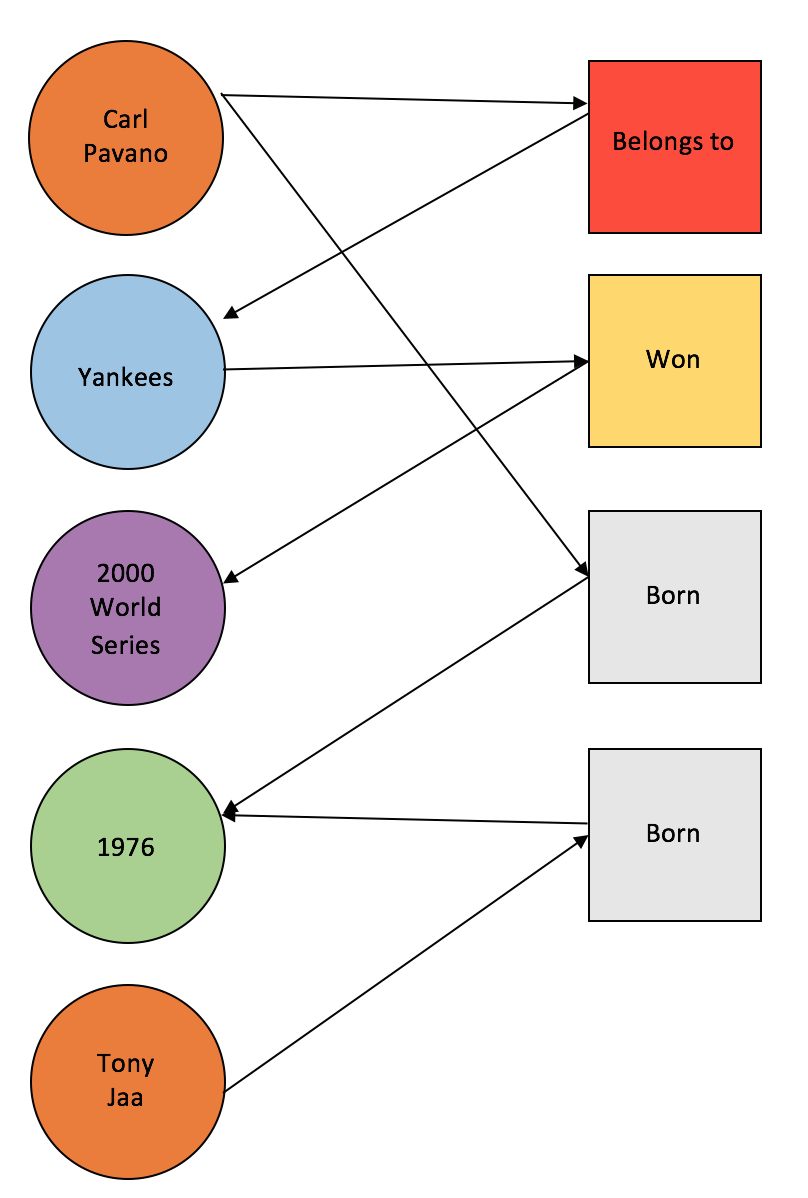
\includegraphics[width=0.7\textwidth,keepaspectratio]{figures/total_dataset_graph.png}
    \caption{An optimal community assignment for four triples in the large dataset}
    \label{fig: total}
\end{figure}

As discussed in Section \ref{Introduction}, community detection algorithms are
very tough to evaluate because there is not necessarily one assignment that is
better than all the others. This ambiguity is why we use the metric of node and
state penalties to find a good assignment. We ran the experiment with varying
numbers of communities, and found that 4 for entities and 4 for relations
yielded the best results. These numbers also make sense intuitively, as there
are 4 sources of data.

Table~\ref{tab: totalE} shows the distribution of entity nodes in each entity
community, along with the set from which each node originated. In the ideal
assignment, each community would have nodes from only one set and all nodes
from each set would be in the same community. Our results are not idea. In fact,
nodes from each set are distributed across all four communities, and within each
community there are nodes from all four sets. Some sets have a better partition
than others. For example, nodes from the Events set are mostly in Communities
1 and 2, with very few in 3 and 4. Similarly, nodes from the People set are
predominantly in Communities 1 and 3. However, for the most part the algorithm
results are suboptimal.

\begin{table}[]
    \begin{tabular}{|c||c|c|c|c|}
        \hline
        & Community 1 & Community 2 & Community 3 & Community 4 \\ \hline
        Language & 6 & 5 & 10 & 6 \\ \hline
        Events & 12 & 12 & 3 & 6 \\ \hline
        People & 42 & 33 & 42 & 37 \\ \hline
        Sports & 22 & 26 & 21 & 15 \\ \hline
    \end{tabular}
    \label{tab: totalE}
    \caption{Table of Entity Communities in the large dataset}
\end{table}

Table~\ref{tab: totalR} shows the distribution of relation nodes in each
relation community, along with the set from which each node originated. The
results are about the same as with the entity communities. While the Events set
is mostly in Communities 1 and 3, for the most part the communities do not
match the optimal assignment.

\begin{table}[]
    \begin{tabular}{|c||c|c|c|c|}
        \hline
        & Community 1 & Community 2 & Community 3 & Community 4 \\ \hline
        Language & 86 & 84 & 88 & 78 \\ \hline
        Events & 76 & 65 & 76  & 71 \\ \hline
        People & 441 & 399 & 395 & 413 \\ \hline
        Sports & 252 & 263 & 215 & 246 \\ \hline
    \end{tabular}
    \label{tab: totalR}
    \caption{Table of Relation Communities in the large dataset}
\end{table}

\subsection{Discussion}
\label{Discussion}

The algorithm's performance on the two datasets demonstrates that it works quite
well for smaller datasets, but becomes less accurate as the size increases. This
decrease in accuracy is most likely due to the fact that entity communities depend
on the relation communities being accurate, and vice versa. The intuition behind
the algorithm is that the iterative nature would allow both classes to improve
simultaneously. In practice, however, instead of mutually becoming more accurate
they mutually stay inaccurate.

The low accuracy on larger datasets is also counterintuitive because we expect
the larger datasets to be denser, and therefore the algorithm should be able to
assign nodes to communities more accurately. In a denser knowledge graph each
entity node appears in many triples, which allows the algorithm to better
categorize each node based on the types of relations it is involved with. On the
other hand, a smaller and sparser graph can suffer from noise. For example, in
Figure~\ref{fig: Colored_Bipartite_KG} if Rita Wilson did not have a \textit{has
spouse} relation and only the \textit{has profession} relation, then that node
only has two edges in common with the Tom Hanks node. The fewer edges in common
it has with another node, the less likely it is that the algorithm will put
those two nodes in the same community. The algorithm takes a longer time to
converge on dense graphs, however.

The number of communities specified can also greatly affect the algorithm's
accuracy. As discussed earlier, there is not necessarily a clear reason why
any particular number should be specified. The most robust way of choosing is
to run for many values and see which has more optimal results.

\subsection{Future Improvements}
\label{Future Improvements}

There are various ways in which this algorithm could be modified to have higher
accuracy. One modification is to have more accurate initializations, instead of
simply randomly assigning nodes to communities at the start. The problem with
random initializations is that different initial states could lead to very
different outcomes. Additionally, some initial states are far worse than others
so the algorithm must be run with many different initializations. We compared
our algorithm to WALKSAT in Section \ref{Similarity to other AI Algorithms}, and
adding more accurate initializations would make it even more like WALKSAT. There
are heuristics that official WALKSAT implementations use to initialize
assignments. Such an improvement could be made to our algorithm as well.

Another possible improvement is to allow the number of communities to be dynamic,
rather than specified beforehand. The algorithm itself would need to be modified
to take into account creating a new community or emptying an existing one. The
current state penalty is defined in such a way that if every node is in its own
community the total penalty is 0. There would need to be an extra penalty for
the total number of communities, to incentivize the algorithm to keep the
total number small.

The third improvement is to add supervision to the algorithm training process.
An unsupervised algorithm is more easily generalizable, but adding some supervision
could help increase the accuracy. The most logical way is to only perform community
detection on the entity side, while specifying the relation types as an input
to the algorithm. If the relation communities are already ideal, the algorithm
should be able to detect entity communities. Most other knowledge graph algorithms
\cite{Nickel2011}\cite{Gao2015}\cite{Chang2014} provide full labels as well as
categorical information, so even just providing the relation communities would
still be relatively unsupervised.

\section{Conclusion}
\label{sec:Conclusion}

In this paper we present a fast, unsupervised community detection algorithm. The
algorithm is an iterative algorithm which assigns penalties to nodes. These
penalties reflect how similar a node's edges are to the edges of other nodes  in
its own community. Although the algorithm does not perform as well as hoped, it
does meet the initial goals of this research. This algorithm is fast in that it
is almost linear time per iteration, and it is also completely unsupervised. The
community detection is not very accurate, but it does serve as a good starting
point. We present three possible modifications that could improve the accuracy
of the algorithm.

\end{document}
